%-------------------------PRÉ_ÂMBULO-------------------------------------------
\documentclass[dvipdfm, a4paper, 11pt]{report}
\usepackage[brazil]{babel}
\usepackage{url}
\usepackage[utf8]{inputenc}
\usepackage{amssymb, amsmath, pxfonts}
\usepackage[normalem]{ulem} %permite sublinhar palavras
\usepackage{mathrsfs} %permite o uso de letras trabalhadas
\usepackage{graphicx}
\usepackage[usenames]{color}
\usepackage{listings}
\usepackage[]{algorithm2e} %para algoritmos
\usepackage{verbatim}%verbatim e comment
%--------------------------------------------------------------------------------
\pagestyle{empty}

\begin{document}



\vspace*{-4cm} \hspace*{-1cm} {\small
{\mbox{\begin{minipage}[t]{2.0cm}
\centerline{
\includegraphics[scale=0.25]{unimontes.eps}}
\end{minipage}}} \hspace*{1cm}
\begin{minipage}{12.0cm}{\sf \large \textbf{UNIVERSIDADE ESTADUAL DE MONTES CLAROS}}\\
{\sc Centro de Ciências Exatas e Tecnológicas}\\
{\sc Engenharia de Sistemas}\\
\end{minipage}
 \vspace*{-3mm}

\vspace{3.5cm}

\begin{center}
\LARGE{ \textbf{Sinais e Sistemas}}
\end{center}

\vspace{4cm}

\begin{center}
\huge{ \textbf{2$^o$ Trabalho}}
\end{center}

\vspace{5cm}

\Large{\uline{Luana Michelly Aparecida da Costa}}
\vspace{4cm}
\begin{center}
\normalsize{Montes Claros, 27 de maio de 2015}
\end{center}
\newpage
\normalsize{\tableofcontents }

\chapter{Introdução}\label{intro}

\section{Proposta do Trabalho}
\subsection{Função de convolução de dois sinais}
Implementar uma função que realize a convolução entre dois sinais de tempo discreto. A função
deve receber como parâmetros de entrada os dois sinais (numpy arrays) e o valor inicial da
variável independente(já que o sinal de saída somente começará a aparecer quando os dois sinais se "encontrarem", a função trabalha a partir deste ponto) e retornar o sinal resultante (numpy array) e os respectivosvalores da variável independente (numpy array).

\subsection{Realizar testes com alguns sinais}
Realize testes com alguns sinais (escolha os sinais que julgar serem interessantes), apresentando
sempre três gráficos:\\
\begin{itemize}
	\item Os sinais de entrada,
	\item O sinal resultante da convolução.
\end{itemize}
\section{Objetivos}
O objetivo principal deste trabalho, segundo o professor, é permitir que a acadêmica, 
por meio da utilização de uma ferramenta computacional, consiga compreender 
a interpretação “rebate, desloca, multiplica e soma” do somatório de convolução. 
Como objetivo secundário, tem-se o incentivo ao estudo da linguagem Python.
Além disso, toma-se como objetivo da acadêmica a continuação do estudo do \LaTeX.

\section{Descrição do Problema}\label{desc}
\subsection{Representação de sinais de tempo discreto em termos de impulsos}

\subsection{A resposta ao impulso e a representação da Soma de Convolução dos Sistemas LIT(Lineares e Invariantes no Tempo)}

\chapter{Desenvolvimento}\label{desenv}

\section{Passando a ideia da solução com pseudocódigo}
Ao analisar como é formado o vetor resultante da convolução de dois sinais, pôde-se montar mais claramente um algoritmo para realizar tal função, segue abaixo o pseudo-código comentado:\\
\\
\begin{algorithm}[H]
\begin{comment}
******** Basic commands for algorithm:
\STATE <text>
 \IF{<condition>} \STATE{<text>} \ELSE \STATE{<text>} \ENDIF
 \FOR{<condition>} \STATE{<text>} \ENDFOR
 \FOR{<condition> \TO <condition> } \STATE{<text>} \ENDFOR
 \FORALL{<condition>} \STATE{<text>} \ENDFOR
 \WHILE{<condition>} \STATE{<text>} \ENDWHILE
 \REPEAT \STATE{<text>} \UNTIL{<condition>}
 \LOOP \STATE{<text>} \ENDLOOP
 \REQUIRE <text>
 \ENSURE <text>
 \RETURN <text>
 \PRINT <text>
 \COMMENT{<text>}
 \AND, \OR, \XOR, \NOT, \TO, \TRUE, \FALSE
\end{comment}

\end{algorithm}

\section{Explicando o algoritmo passo a passo}

\small{
\begin{lstlisting}[language = python]
def Conv(x,h,valor_inicial):
	#Inicializando algumas variaveis
	lenx = len(x)
	lenh = len(h)
	indep_values = np.arange(valor_inicial, valor_inicial+lenh+lenx-1,1)
	#Mantem o tamanho do vetor, independente do valor_inicial
	y = np.zeros(lenh+lenx-1)
	for i in range(lenh):
		for j in range(lenx):
			y[i+j] = y[i+j] + (h[i]*x[j]) 
		#a medida em que os sinais vao se "interceptando", 
		#o valor de y se atualiza
	return (y, indep_values)

\end{lstlisting}
}
\section{A escolha dos casos teste}

Ao todo foram montados seis casos teste. Em parte aleatórios, mantendo preservado o objetivo inicial ao escolhê-los.
De 1 a 3, os testes variam o tempo inicial entre negativo, positivo e nulo, respectivamente. Os outros visam corroborar 3 das propriedades da convolução. O número 4 ratifica a propriedade comutativa, o 5, a distributiva e o 6 o impulso como elemento neutro da convolução.

\chapter{Resultados}\label{result}
Primeiramente os vetores foram convoluídos pelo software Matlab para efeito de comparação e validação dos resultados.
\section{Resultados obtidos pelo Matlab}

\section{Gráficos gerados pelo algoritmo}
As dimensões dos gráficos foram pseudo-aleatórias, respeitando que os valores resultantes deveriam aparecer.\\
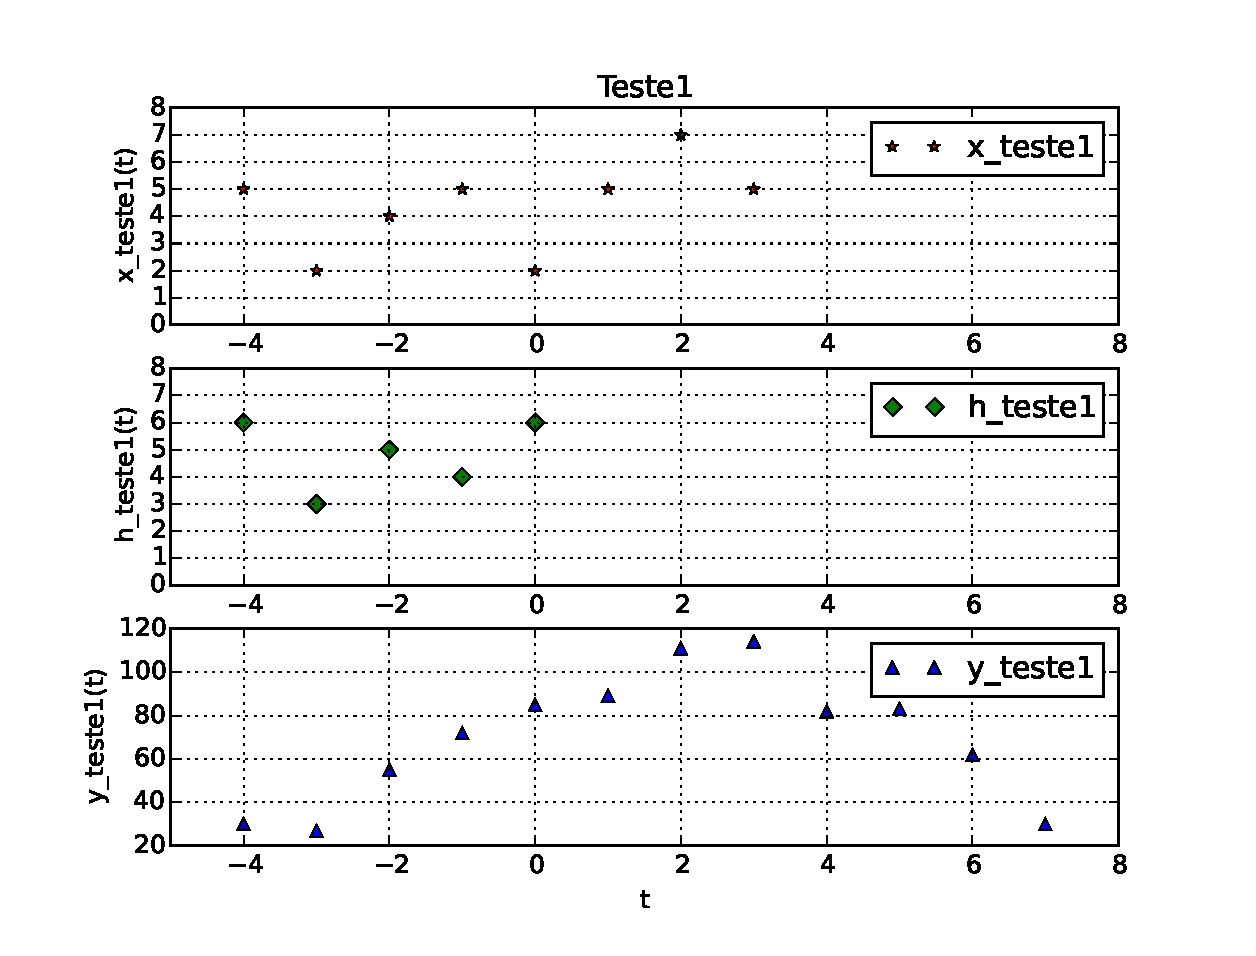
\includegraphics[scale = 0.5]{Teste1.eps}\\
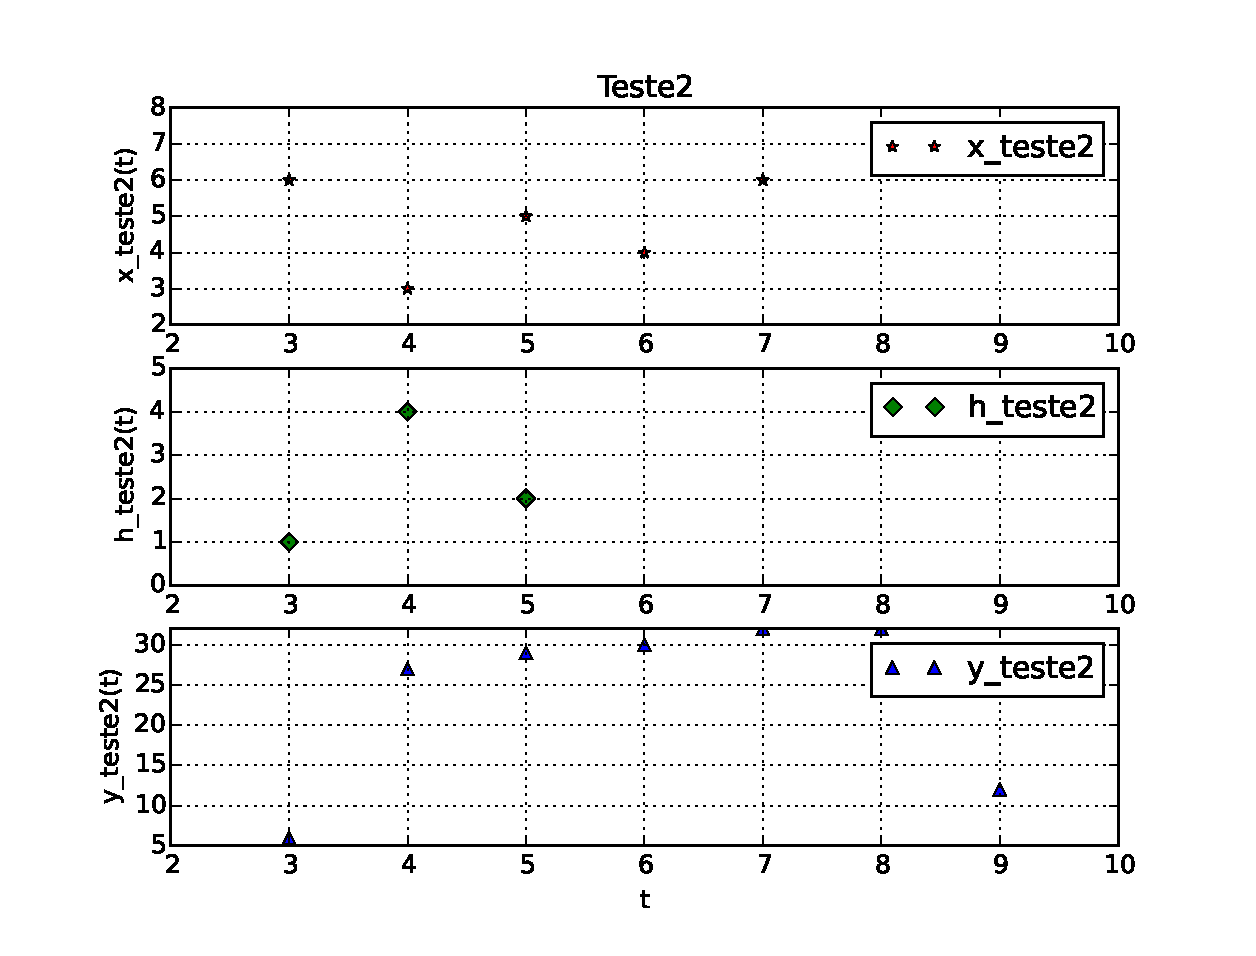
\includegraphics[scale = 0.5]{Teste2.eps}\\
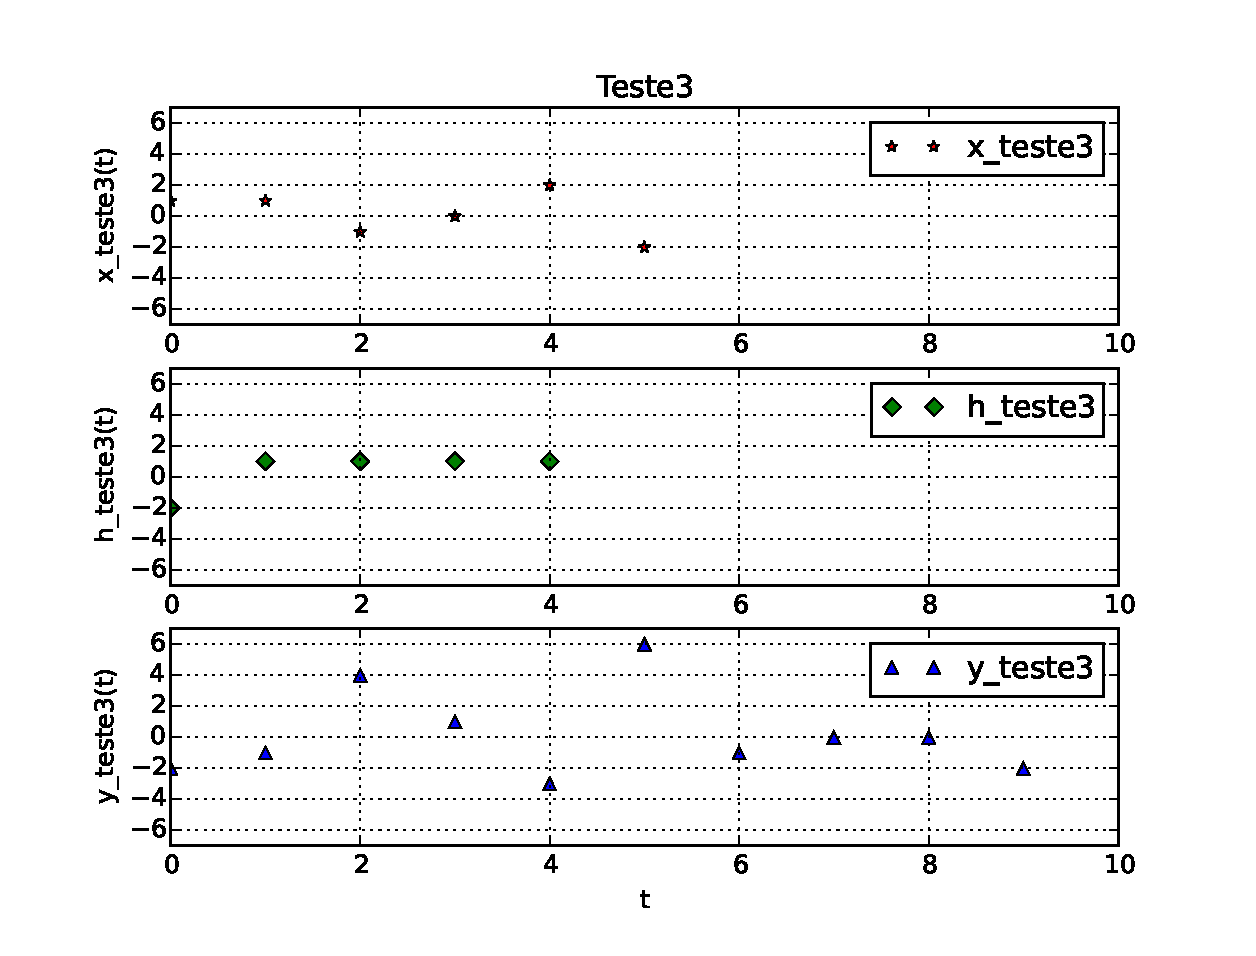
\includegraphics[scale = 0.5]{Teste3.eps}\\
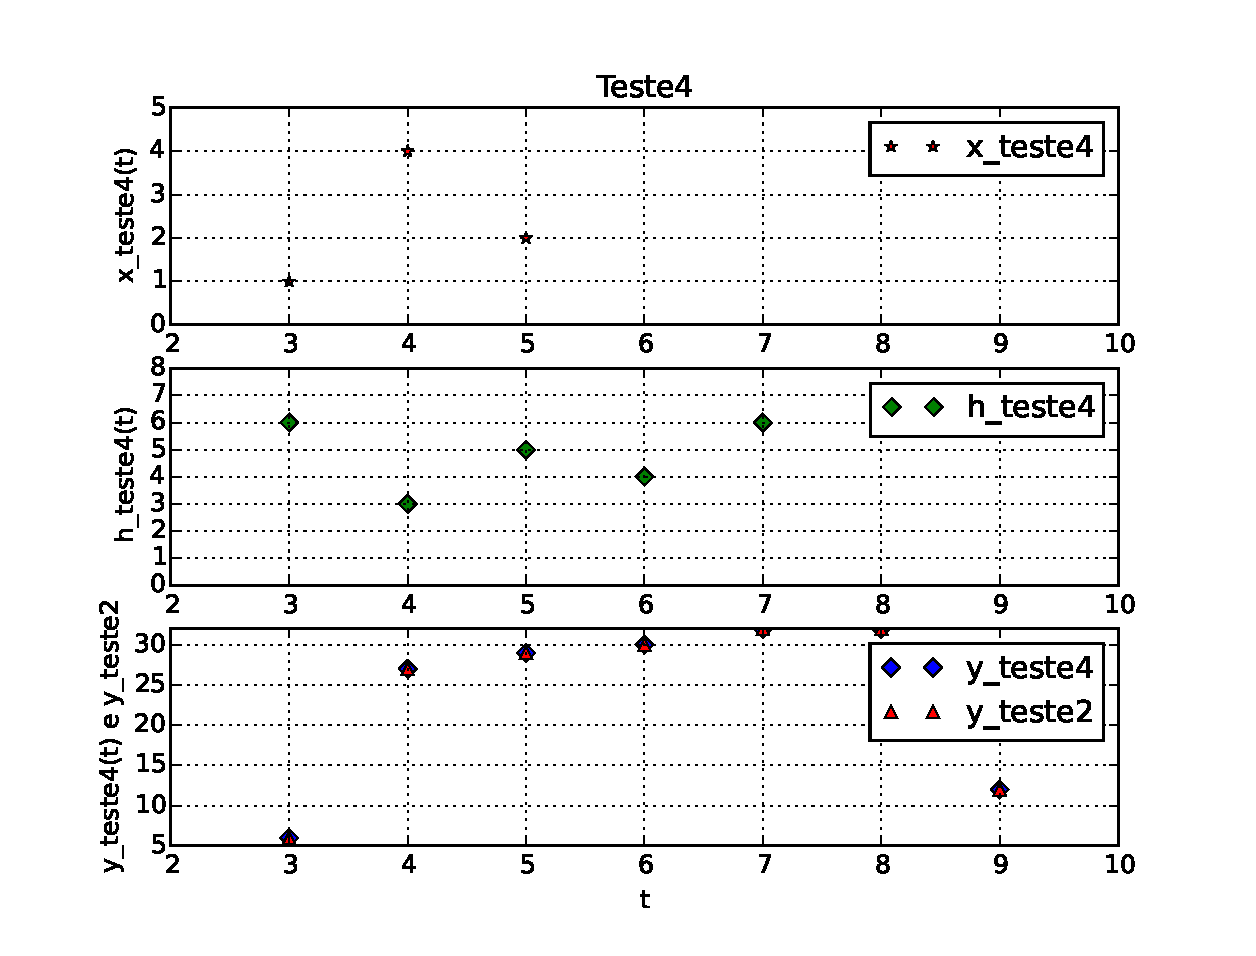
\includegraphics[scale = 0.5]{Teste4.eps}\\
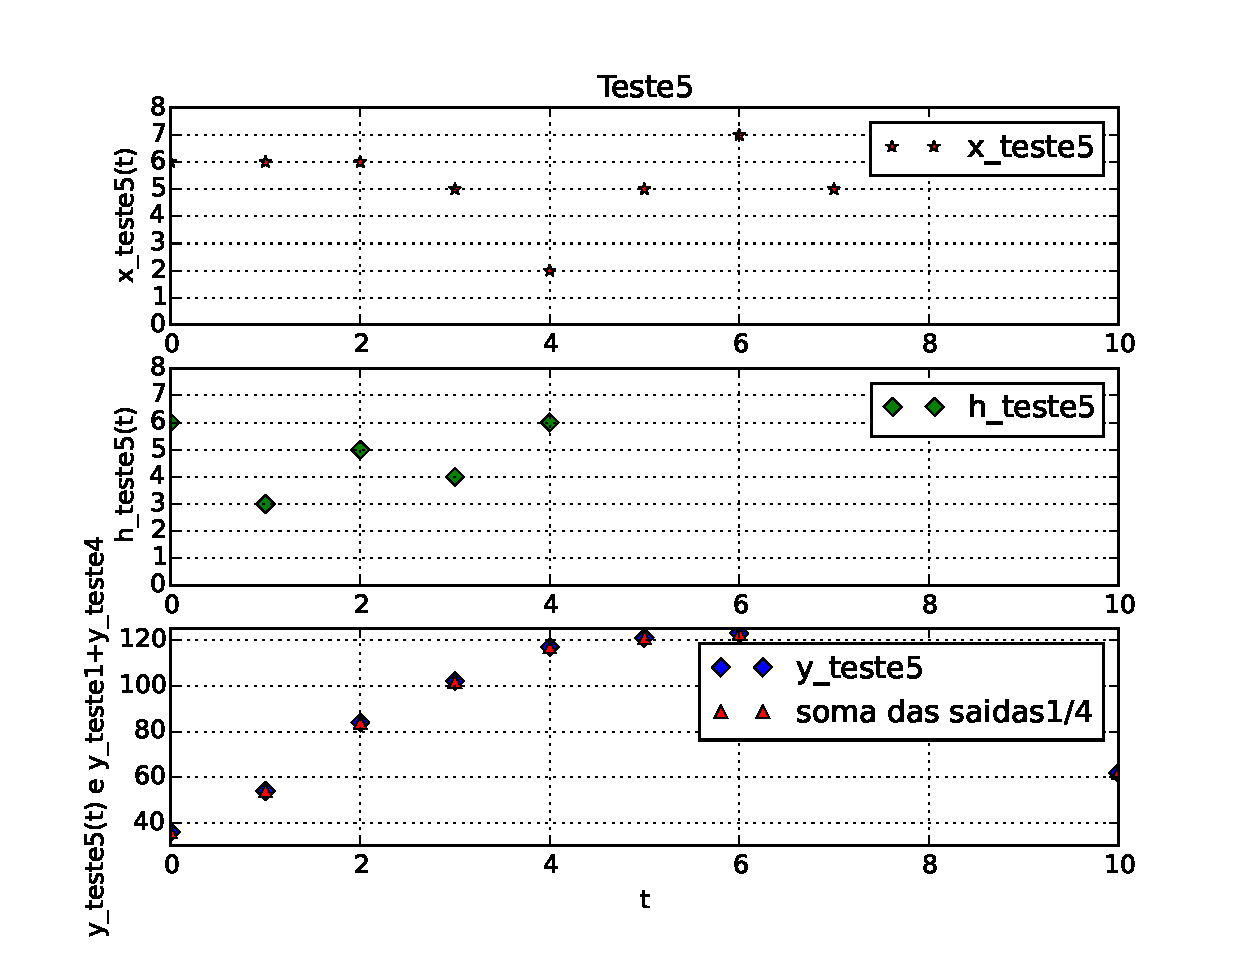
\includegraphics[scale = 0.5]{Teste5.eps}\\
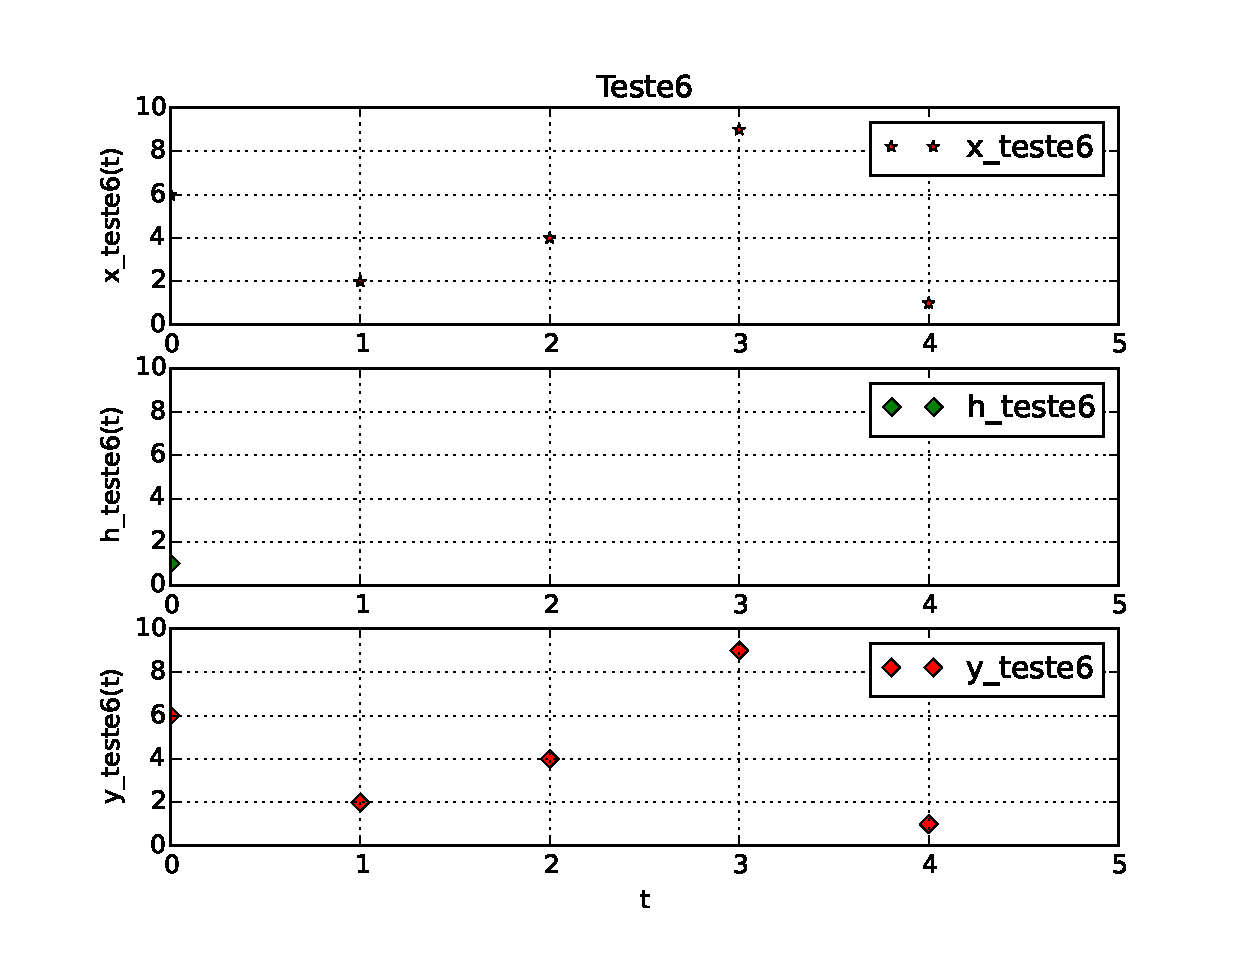
\includegraphics[scale = 0.5]{Teste6.eps}\\
\chapter{Conclusão}\label{conc}
De acordo com os resultados apresentados durante o desenvolvimento da documentação, pode-se afirmar que todos os objetivos foram cumpridos.
Quanto à elaboração da função, ela funciona adequadamente, gerando os gráficos correspondentes. O estudo das linguagens \emph{Python} e \LaTeX vem elevando para que o trabalho possa ser desenvolvido da melhor maneira possível.

\begin{thebibliography}{999}
\small{
\bibitem{np} NumPy Reference. Disponível em: $<$\url{http://docs.scipy.org/doc/numpy/reference/index.html}$>$. Acesso em: 18 de maio de 2015. 
\bibitem{matplot} Matplotlib Reference. Disponível em: $<$\url{http://matplotlib.org/contents.html}$>$. Acesso em: 18 de maio de 2015.
\bibitem{Opp} OPPENHEIM, A.V.;WILLSKY,A.S.;NAWAB,S.H.\emph{Signals and Systems}. 2th edition.
\bibitem{Haykin} HAYKIN, S.; VEEN,B.V. \emph{Sinais e Sistemas}. Tradução: José Carlos Barbosa dos Santos. Porto Alegre, 2001
\bibitem{wolfram} Demonstração da Soma de Convolução em formato "*.cdf". Wolfram Demonstrations Project.
\bibitem{site} Vetores e matrizes com numpy. Disponível em: $<$\url{http://www.pbx-brasil.com/Pesquisa/Ferramentas/ProgramandoPython/aula112/vetoresNumpy.html}$>$. Acesso em: 18 de maio de 2015.
\bibitem{pdfaula1} Sistemas lineares e Invariantes. Universidade do Porto, Faculdade de Engenharia, 2007/2008.$<$\url{http://paginas.fe.up.pt/~mines/SS/Teoricas/SLITs/SS_slits_aula1.pdf}$>$. Acesso em: 18 de maio de 2015.
\bibitem{python_flavio}Computação científica com Python. Disponível em: $<$\url{http://www.complex.if.uff.br/_media/python_flavio.pdf}$>$. Acesso em  18 de maio de 2015.
\bibitem{mathworks}Documentação da função \textit{conv} do Matlab. Dis $<$\url{http://www.mathworks.com/help/matlab/ref/conv.html}$>$. Acesso em: 18 de maio de 2015.
\bibitem{wiki}Convolução.Disponível em: $<$\url{http://pt.wikipedia.org/wiki/Convolução}$>$. Acesso em: 18 de maio de 2015.
\bibitem{miles}MILES. Not-So-Frequently Asked Questions for \LaTeX, 2010. Disponível em: $<$\url{http://web.mit.edu/rsi/www/pdfs/ifaq.pdf}$>$ . Acesso em: 24 de maio e 2015.
\bibitem{wikibooks}Wikibooks-\LaTeX. Disponível em: $<$\url{http://en.wikibooks.org/wiki/LaTeX}$>$. Acesso em: 24 de maio de 2015.
\bibitem{brito}BRITO, Rafael.The algorithms bundle, 2009. Disponível em: $<$\url{http://repositorios.cpai.unb.br/ctan/macros/latex/contrib/algorithms/algorithms.pdf}$>$. Acesso em: 24 de maio de 2015.
}
\end{thebibliography}
\end{document}



